\subsection{Ions}
In order to effectively trap an Ion, we use a field that forms a saddle, but rotates constantly so that effectively we see a potential (averaged over a time period):
\begin{align*}
	V &= \frac{m\omega_x^2}{2} x^2 + \frac{m\omega_y^2}{2}y^2 + \frac{m\omega_z^2}{2}z^2
\end{align*}
We choose a special axis by saying $\omega_x = \omega_y \gg \omega_z$. This means that the Ions are free to move along the z axis, but we say they are too strongly trapped to move in $x$ or $y$.
The system can't be in an excited $x$ or $y$ state because $\hbar\omega_x \gg k_B T$, so our atom is very unlikely to be found in that state.

In order to use an Ion as a qubit we can look at various degrees of freedom. Since we typically use atoms with 2 valence electrons, with one removed to ionize it, we can look at this in terms of the hydrogen atom, and use atomic spin to split, as we did with neutral atoms.
But Ions give us access to a new state, which is the $D$ state. For an Ion the $4S$ state which is normally below the $3D$ state gets pushed below the $3D$ state, so we can in fact work the $3D$ state as our excited state.
This energy shift occurs since the screening effect decreases as you get closer, the $D$ states normally see less screening and therefore see less charge, but for the ions we have a larger base charge so the change from decreased screening is less important.
Addionally of note is the fact that the transition here is a quadrapole transition, which should make this a more long lived state (though this transition is harder to drive). \\
\begin{figure*}[h]
	\centering
	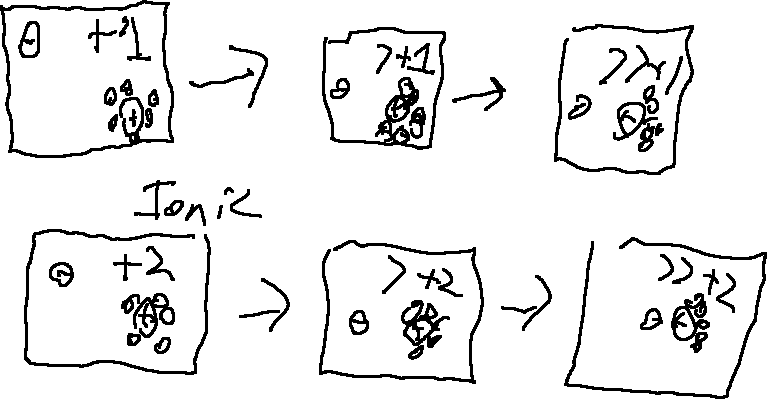
\includegraphics[width=12cm]{11-25-1.png}
	\caption*{A diagram of screening for a neutral atom and an ion}
\end{figure*}
If we look at the quadrapole transition, in order for a single photon to excite the transition we need to have the absorbed photon to have a unit of orbital angular momentum as well as spin angular momentum.

Looking at single qubit gates on an Ion we first say we can certainly use the same scheme for single qubit operations as we did for neutral atoms. If we now consider three ions in the same linear trap, these Ions should all interact with eachother via Coulomb forces.
This is because the Ions have a positive charge, so they should all repel. Clearly as we know from studying coupled harmonic oscilators, we should have several modes that our ions should be able to move in if their overall motion is excited (one mode per ion).
The lowest frequency mode should always be the center of mass motion of the ions, and then the breathing mode should be the first excited mode. If we represent our total center of mass motion with an ancilory qubit (or potentially Fock state).
We can then cause a transition at $\omega_0 + \omega_c$ (where $\omega_c$ is the frequency of the center of mass motion) which would cause a transtion from the $\ket{00}$ state (where the second qubit represents the COM state), to $\ket{11}$.
We can use all this to create a two qubit gate.
\begin{figure*}[h]
	\centering
	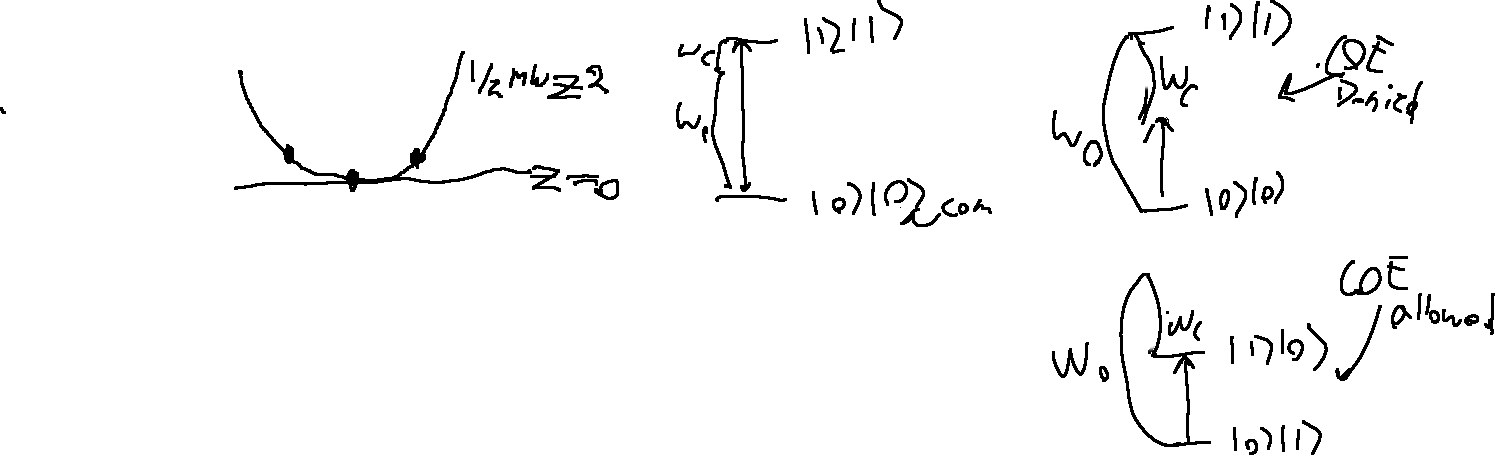
\includegraphics[width=12cm]{11-25-2.png}
	\caption*{Diagram showing the COM motion in relation to state transitions}
\end{figure*}
In order to create our controlled z gate, we first drive a $\pi$ pulse at $\omega_0 - \omega_c$ on our first qubit, then a $2\pi$ pulse on our second qubit at $\omega_0 - \omega_c$, and then finally another $\pi$ pulse on the first atom.
This all works terrifically, but it requires that our initial state has no phonons in the center of mass modes to begin with. This is a cooling process as the energy in the system will be lower after we've forced our system to have no COM phonons.
Since this process needs to be irreversible we want it to use spontaneous emission. If we repeatedly cause stimulated absorption at $\omega_0 - \omega_c$, then wait for spontaneous emission in the excited state, we can see this process will look like:
$\ket{0,n}\to\ket{1,n-1}\to\ket{0,n-1}$. Eventually we should reach a point where there are no remaining phonons, so we will be in the $\ket{1,0}$ state. In actuality we don't switch the laser on and off, and instead run it continously.
This process is known as sideband cooling.
